%\documentclass[crop,tikz,convert={outext=.svg,command=\unexpanded{pdf2svg \infile\space\ou
%tfile}},multi=false]{standalone}[2012/04/13]

\documentclass[crop,tikz]{standalone}[2012/04/13]

\usepackage{pgf}

\usetikzlibrary{arrows,automata}
\usepackage[latin1]{inputenc}
\begin{document}
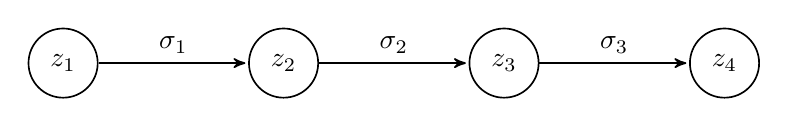
\begin{tikzpicture}[->,>=stealth',shorten >=1pt,auto,node distance=2.8cm,
                    semithick]
 % \tikzstyle{every state}=[fill=red,draw=none,text=white]

  \node[state]         (A)                    {$z_1$};
  \node[state]         (B) [right of=A] {$z_2$};
  \node[state]         (C) [right of=B] {$z_3$};
  \node[state]         (D) [right of=C]       {$z_4$};
  
  \path (A) edge              node {$\sigma_1$} (B);
  \path (B) edge              node {$\sigma_2$}  (C);
  \path (C) edge              node {$\sigma_3$} (D);
\end{tikzpicture}

\end{document}